% !TeX spellcheck = es_ES
\documentclass[12pt, titlepage]{article}
\usepackage[nottoc,notlot,notlof,numbib]{tocbibind}
\usepackage[letterpaper, margin=2.5cm]{geometry}
\usepackage[utf8]{inputenc}
\usepackage[spanish]{babel}
\usepackage{listings}
% imagenes
\usepackage{graphicx} 
\usepackage{float}
% fin imagenes
\usepackage{url}
\usepackage{color}
\usepackage{amsmath}
\usepackage{bm}

\definecolor{dkgreen}{rgb}{0,0.6,0}
\definecolor{gray}{rgb}{0.5,0.5,0.5}
\definecolor{mauve}{RGB}{253,151,31}
\definecolor{deepred}{RGB}{249,38,114}

\lstset{frame=tb,
	language=MATLAB,
	aboveskip=3mm,
	belowskip=3mm,
	showstringspaces=false,
	columns=flexible,
	numbers=left,
	stepnumber=1,
	basicstyle={\small\ttfamily},
	numberstyle=\tiny\color{gray},
	keywordstyle=\color{blue},
	commentstyle=\color{dkgreen},
	stringstyle=\color{mauve},
	breaklines=true,
	breakatwhitespace=true,
	tabsize=2,
	morekeywords={self, append},
	emph={},
	emphstyle=\color{deepred}
}

\title{Reporte de la red ADALINE}
\author{Barrera Pérez Carlos Tonatihu \\Boleta: 2016630023\\ Profesor: Moreno Armendariz Marco Antonio \\ Redes Neuronales \\ Grupo: 3CM2 }

\begin{document}
    \maketitle
    \tableofcontents
    \newpage
    \section{Introducción}
    Este reporte es sobre la red neuronal ADALINE. Se incluye una breve explicación sobre esta red así como su arquitectura, el como funciona y su representación matemática para que sea fácil de entender.
    \\\\
    Asimismo, se programo esta red en dos versiones, una con bias el cual recibe un conjunto de entrenamiento mediante un archivo de texto y otra sin bias que resuelve el problema del codificador, sujeta a algunas restricciones para que fuera más sencilla su elaboración, el desarrollo de estos programas fue realizado en \emph{MATLAB} ya que nos proporciona un manejo sencillo de matrices, lo cual es el principal elemento con el que trabaja esta red neuronal. 
    \\\\
    Para verificar el correcto funcionamiento de los programas se realizaron pruebas con entradas de diferentes tamaños y valores, de igual forma se muestra en pantalla el resultado y una representación gráfica. Para complementar los resultados obtenidos se incluye un análisis de lo que se pudo observar y el porque se obtuvieron dichos resultados.
    \\\\
    Finalmente, tenemos una sección de conclusiones donde se habla sobre la importancia de esta red al igual que sus posibles aplicaciones y ventajas con base en los resultados obtenidos en la sección de experimentos.
    \newpage
    \section{Marco teórico}
    La red ADALINE (ADAptive LInear NEuron) es muy similar a al perceptron con la diferencia que la función de transferencia es lineal en lugar de ser escalón esto se puede observar en la figura \ref{fig:adaline-diagrama}, y al igual que el perceptron solo pueden resolver problemas linealmente separables como por ejemplo el problema de la compuerta AND de la figura \ref{fig:AND}. \cite{pagina}
    \begin{figure}[H]
        \begin{center}
            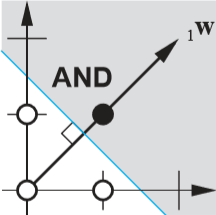
\includegraphics[width=5cm]{img/adaline/AND.png}
            \caption{La compuerta AND es linealmente separable. \cite{libro1}}
            \label{fig:AND}
        \end{center}
    \end{figure}
    Por otro lado un problema linealmente no separable seria el de la figura \ref{fig:XOR} ya que no es posible trazar lineas que funjan como frontera de decision entre las dos clases que tenemos.
    
    Otro aspecto importante de ADALINE es que el algoritmo LMS es mas poderoso que la regla de aprendizaje del perceptron. Esto debido a que la regla de aprendizaje del perceptron garantiza la convergencia a una solución que clasifica los vectores prototipo. Por lo que es sensible al ruido que se produce debido a que estos vectores suelen estar muy cerca de las fronteras de decisión.
    \begin{figure}[H]
        \begin{center}
            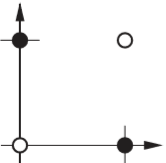
\includegraphics[width=5cm]{img/adaline/XOR.png}
            \caption{La compuerta XOR no se puede separar linealmente. \cite{libro1}}
            \label{fig:XOR}
        \end{center}
    \end{figure}
    Este problema es solucionado con LMS, el cual desplaza las fronteras de decisión lejos de los patrones de entrenamiento esto vuelve a este método más útil y aplicable a otros campos como el procesamiento de señales digital de señales en donde se utiliza para cancelar echo en las lineas telefónicas de larga distancia.
    
    La arquitectura de esta red es la siguiente.
    \begin{figure}[H]
        \begin{center}
            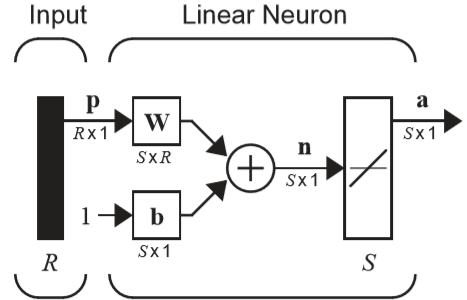
\includegraphics[width=9cm]{img/adaline/arquitectura.png}
            \caption{Arquitectura de la red ADALINE. \cite{libro1}}
            \label{fig:adaline-diagrama}
        \end{center}
    \end{figure}
    Se puede apreciar su similitud con el perceptron incluso en la ecuación que produce la salida de la red, la cual está definida como.
    \[ \boldsymbol{a = purelin(Wp+b)} \]
    Esta red es entrenada por aprendizaje supervisado por lo que utilizamos un conjunto de entrenamiento y el algoritmo LMS que se encarga de ajustar los pesos y bias con el objetivo de minimizar el error medio cuadrático.
    \[ \left\lbrace \boldsymbol{p_1, t_1}\right\rbrace , \left\lbrace \boldsymbol{p_2, t_2}\right\rbrace , ... , \left\lbrace \boldsymbol{p_Q, t_Q}\right\rbrace\]
    El algoritmo es el siguiente. \cite{otro}
    \begin{enumerate}
        \item Inicialización de los pesos y bias de forma aleatoria.
        \item Se aplica un patrón $p_Q$ de entrada.
        \item Se computa una salida lineal utilizando la red.
        \item Se calcula el error cometido por la red para dicho patrón el cual se calcula de la siguiente forma.
        \[\boldsymbol{e_Q = t_Q - a_Q} \]
        donde $\boldsymbol{e_Q}$ es el error, $\boldsymbol{t_Q}$ es el vector objetivo y $\boldsymbol{a_Q}$ es la salida que produce la red.
        \item Se actualizan los pesos y bias utilizando el error obtenido en el paso anterior de la siguiente forma.
        \begin{gather*}
        \boldsymbol{W}(k+1) = \boldsymbol{W}(k) +2\alpha \boldsymbol{e}(k)\boldsymbol{p^T}(k) \\
        \boldsymbol{b}(k+1) =\boldsymbol{b}(k) + 2\alpha \boldsymbol{e}(k)
        \end{gather*}
        donde $\boldsymbol{W}(k+1)$ y $\boldsymbol{b}(k+1)$ son los nuevos valores de nuestros pesos y bias, $\boldsymbol{W}(k)$ y $\boldsymbol{b}(k)$ son los valores actuales, $\alpha$ es un factor de aprendizaje que suele tener valores muy pequeños para evitar modificaciones drásticas en los valores de la red y $\boldsymbol{p^T}(k)$ es la transpuesta de nuestro vector de entrada.
        \item Se repiten los pasos 2 a 5 para todos los patrones de entrenamiento.
        \item Después de esto termina una iteración y se calcula el error cuadrático medio, este error es calculado de la siguiente forma.
        \[ e^2 = \frac{1}{Q} \sum _{i=1}^{Q} e^2_i \]
        Si el error cuadrático medio es un valor reducido aceptable o hemos alcanzado un máximo de iteraciones terminamos el proceso, de lo contrario se vuelve al paso 2.
    \end{enumerate}
\newpage
    \section{Resultados experimentales}
    Los experimentos en ADALINE consistieron se dividieron en dos partes, la primera para pruebas que involucraran bias en donde se introdujo un archivo con el conjunto de entrenamiento al igual que en el perceptron, y por otro lado para la parte en la que no se utilizo el bias sólo se resolvió el problema del codificador en el cual el usuario indica el tamaño del codificador y la red comienza a trabajar como lo haría comúnmente.
    
    Ambos tipos de experimentos incluyen la graficación de la evolución del error por iteración y de los valores de pesos y bias, además de que los valores finales son almacenados en un archivo llamado \emph{resultado\_hora\_fecha.txt}
    \begin{figure}[H]
        \begin{center}
            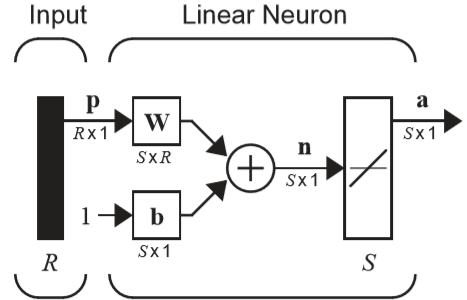
\includegraphics[width=9cm]{img/adaline/arquitectura.png}
            \caption{Arquitectura de la red ADALINE con bias. \cite{libro1}}
            \label{fig:adaline-diagrama2}
        \end{center}
    \end{figure}
    \subsection{Con bias}
    \textbf{Experimento 1}
    El conjunto de entrenamiento que se utilizo en este caso fue.
    \[ \left\lbrace \boldsymbol{p_1} = \left[\begin{array}{c} 0\\ 0\end{array}\right], t_1 = -1  \right\rbrace, \left\lbrace \boldsymbol{p_2} = \left[\begin{array}{c} 0\\ 1\end{array}\right], t_2 = -1  \right\rbrace, \left\lbrace \boldsymbol{p_3} = \left[\begin{array}{c} 1\\ 0\end{array}\right], t_3 = -1  \right\rbrace, \left\lbrace \boldsymbol{p_4} = \left[\begin{array}{c} 1\\ 1\end{array}\right], t_4 = 1  \right\rbrace  \]
    El cual corresponde a una compuerta AND de dos entradas. Esto provoco que los valores asociados a nuestra arquitectura de la figura \ref{fig:adaline-diagrama2} fueran los siguientes.
    \begin{align*}
    S=1 && R=2
    \end{align*}
    Además los valores asociados a $\boldsymbol{W}$ y $\boldsymbol{b}$ fueron números aleatorios pequeños. De igual forma se ingresan los valores para el factores de aprendizaje, número máximo de iteraciones y el mínimo error permitido, $\alpha=.03$, $it_{max}=100$, $e_{it}=.1$ respectivamente.
    \begin{figure}[H]
        \begin{center}
            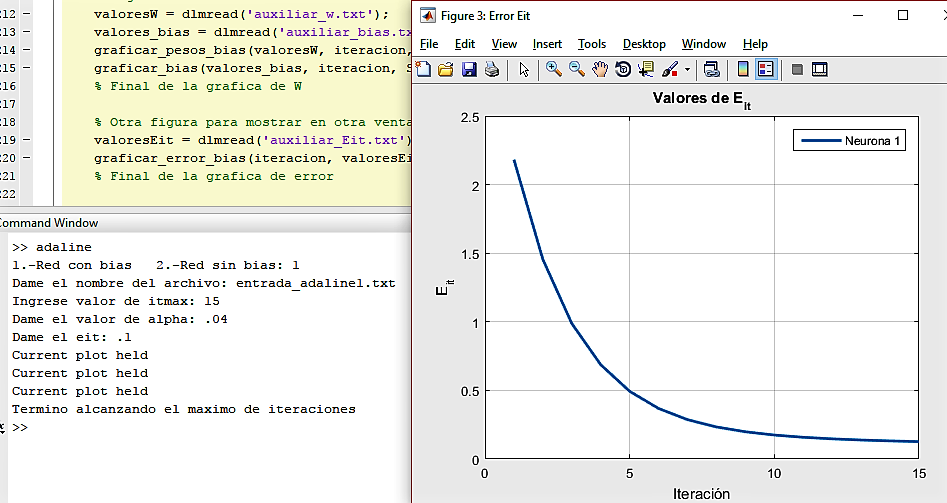
\includegraphics[width=16cm]{img/adaline1/error.png}
            \caption{Prueba 1 de ADALINE con bias.}
            \label{fig:adaline1error}
        \end{center}
    \end{figure}
    En la figura \ref{fig:adaline1error} se puede observar que la red llego a un resultado en la iteración 25 debido al criterio de error menor al permitido por iteración como se ve reflejado en la gráfica correspondiente, dando como resultado los siguientes valores para los pesos y bias.
    \begin{align*}
    \boldsymbol{W} = \left[\begin{array}{cc}0.5744 & 0.5956\end{array}\right] && \boldsymbol{b} = -0.9391
    \end{align*}
    Estos valores son almacenados en su respectivo archivo \emph{resultado\_hora\_fecha.txt}, en la figura \ref{fig:adaline1pesos} se puede observar su evolución a lo largo de las 25 iteraciones.
    \begin{figure}[H]
        \begin{center}
            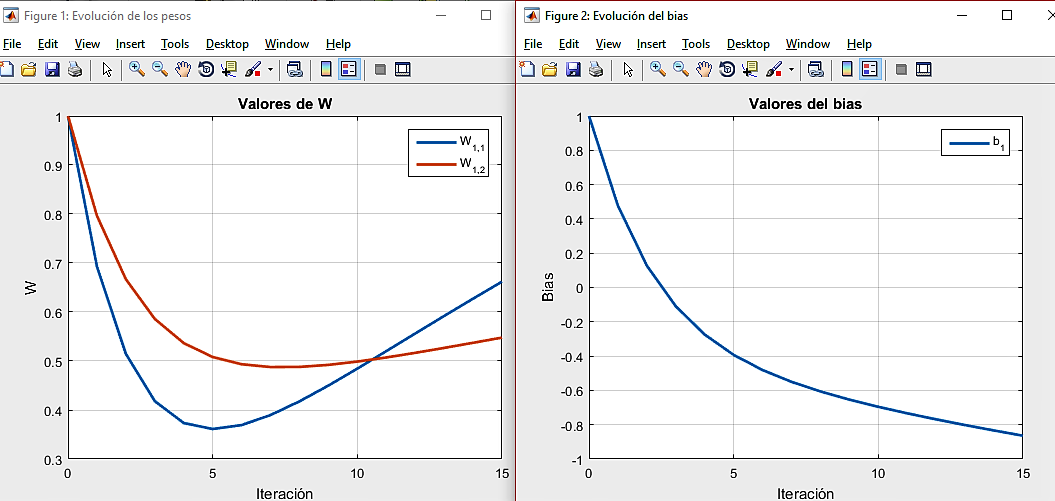
\includegraphics[width=16cm]{img/adaline1/pesosbias.png}
            \caption{Pesos y bias en esta prueba.}
            \label{fig:adaline1pesos}
        \end{center}
    \end{figure}
    \textbf{Experimento 2}
    El conjunto de entrenamiento que se utilizo para entrenar a la red fue.
    \[ \left\lbrace \boldsymbol{p_1} = \left[\begin{array}{c} 1\\ 1\end{array}\right], \boldsymbol{t_1} = \left[\begin{array}{c} -1\\ -1\end{array}\right]  \right\rbrace, \left\lbrace \boldsymbol{p_2} = \left[\begin{array}{c} 2\\ 0\end{array}\right], \boldsymbol{t_2} = \left[\begin{array}{c} -1\\ -1\end{array}\right]  \right\rbrace, \left\lbrace \boldsymbol{p_3} = \left[\begin{array}{c} -1\\ -1\end{array}\right], \boldsymbol{t_3} = \left[\begin{array}{c} -1\\ 1\end{array}\right]  \right\rbrace,\]
    
    \[ \left\lbrace \boldsymbol{p_4} = \left[\begin{array}{c} 0\\ -1\end{array}\right], \boldsymbol{t_4} = \left[\begin{array}{c} -1\\ 1\end{array}\right]  \right\rbrace, \left\lbrace \boldsymbol{p_5} = \left[\begin{array}{c} -2\\ 0\end{array}\right],\boldsymbol{t_5} = \left[\begin{array}{c} 1\\ -1\end{array}\right]  \right\rbrace, \left\lbrace \boldsymbol{p_6} = \left[\begin{array}{c} -1\\ 1\end{array}\right], \boldsymbol{t_6} = \left[\begin{array}{c} 1\\ -1\end{array}\right]  \right\rbrace,\]
    
    \[ \left\lbrace \boldsymbol{p_7} = \left[\begin{array}{c} 0\\ 2\end{array}\right], \boldsymbol{t_7} = \left[\begin{array}{c} 1\\ 1\end{array}\right]  \right\rbrace, \left\lbrace \boldsymbol{p_8} = \left[\begin{array}{c} 1\\ 2\end{array}\right], \boldsymbol{t_8} = \left[\begin{array}{c} 1\\ 1\end{array}\right]  \right\rbrace\]
    Es por estos valores que las dimensiones de la red mostrada en la figura \ref{fig:adaline-diagrama2} quedan definidas de la siguiente forma.
    \begin{align*}
    S = 2 && R = 2
    \end{align*}
    Lo cual crea una matriz de pesos de $2x2$ y una matriz de bias de $2x1$ con valores aleatorios pequeños, mientras que los valores de iteración máxima, factor de aprendizaje y error permitido son de nueva cuenta introducidos manualmente de la forma $it_{max}=20$, $\alpha=0.04$,  $e_{it}=0.1$ respectivamente (véase figura \ref{fig:adaline2error}).
    \begin{figure}[H]
        \begin{center}
            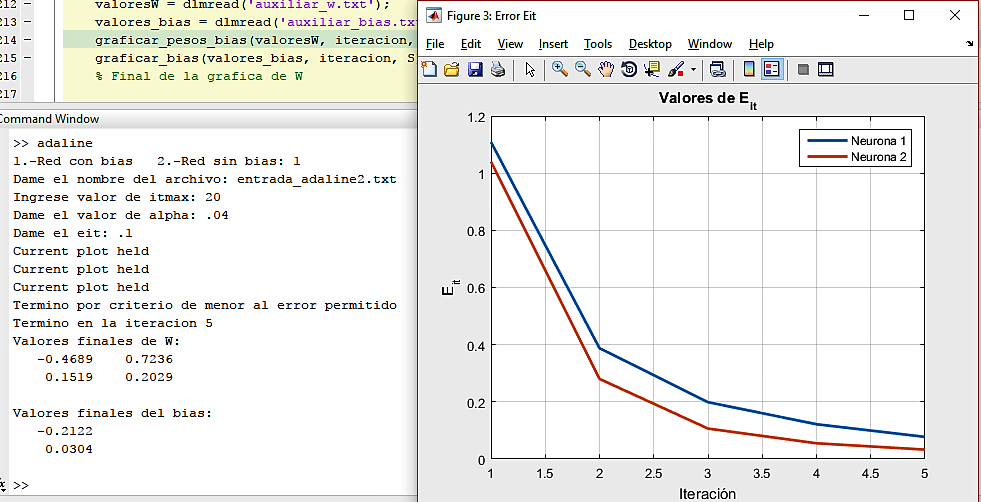
\includegraphics[width=16cm]{img/adaline2/error.png}
            \caption{Prueba 2 de ADALINE con bias.}
            \label{fig:adaline2error}
        \end{center}
    \end{figure}
    En esta ocasión la red convergió en la iteración 5 debido al criterio de menor al error permitido reflejado en la figura \ref{fig:adaline2error} para cada una de las neuronas que componen esta red. Los valores finales de pesos y bias se almacenaron en su correspondiente archivo de salida con los valores.
    \begin{align*}
    \boldsymbol{W} = \left[\begin{array}{cc}-0.4648& 0.7236\\ 0.1519& 0.2029\end{array}\right] && \boldsymbol{b} = \left[\begin{array}{c}-0.2122\\ 0.0304\end{array}\right]
    \end{align*}
    \begin{figure}[H]
        \begin{center}
            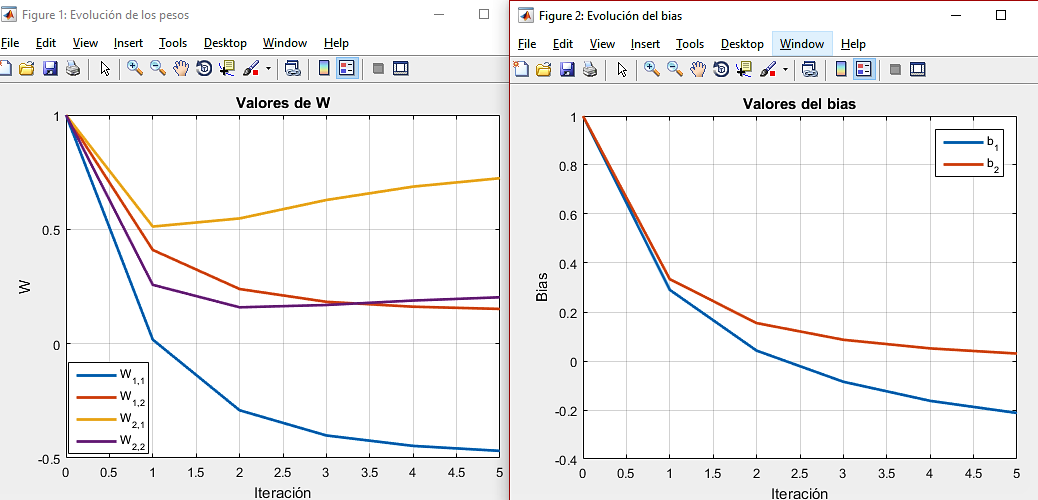
\includegraphics[width=16cm]{img/adaline2/pesosbias.png}
            \caption{Pesos y bias en esta prueba.}
            \label{fig:adaline2pesos}
        \end{center}
    \end{figure}
    \subsection{Sin bias}
    \textbf{Experimento 1}. En este caso el tamaño del codificador ingresado por el usuario fue de 4, el error mínimo aceptable fue $e_{it} = 0.01$ y el valor de alpha fue $\alpha=0.02$, esto se puede observar en la figura \ref{fig:adaline3error}.
    \begin{figure}[H]
        \begin{center}
            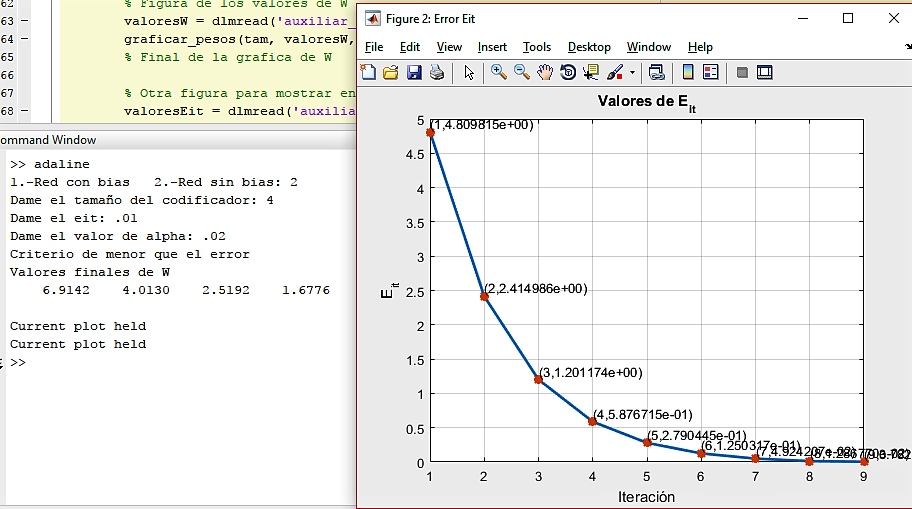
\includegraphics[width=16cm]{img/adaline3/error.png}
            \caption{Prueba 1 de ADALINE sin bias.}
            \label{fig:adaline3error}
        \end{center}
    \end{figure}
    La red convergió en la debido a que el error es menor al valor aceptable dando como resultado los siguientes valores de $\boldsymbol{W}$.
    \[ \boldsymbol{W} = \left[\begin{array}{cccc}6.9142 & 4.0130 & 2.5192 & 1.6776\end{array}\right] \]
    \begin{figure}[H]
        \begin{center}
            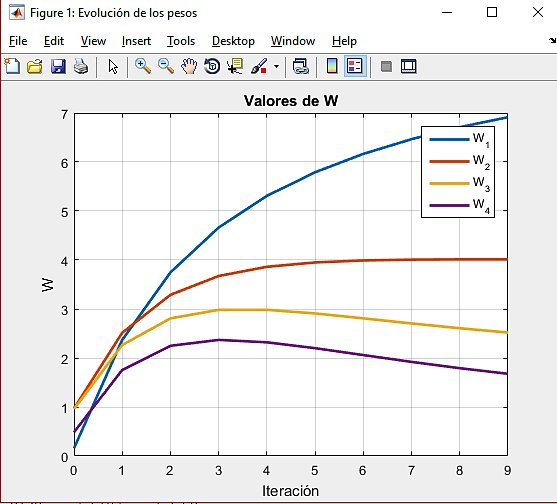
\includegraphics[width=10cm]{img/adaline3/pesosbias.png}
            \caption{Pesos de esta prueba.}
            \label{fig:adaline3pesos}
        \end{center}
    \end{figure}
    \textbf{Experimento 2}. En este caso el tamaño del codificador ingresado por el usuario fue de 5, el error mínimo aceptable fue $e_{it} = 0.01$ y el valor de alpha fue $\alpha=.03$, esto se puede observar en la figura \ref{fig:adaline4error}
    \begin{figure}[H]
        \begin{center}
            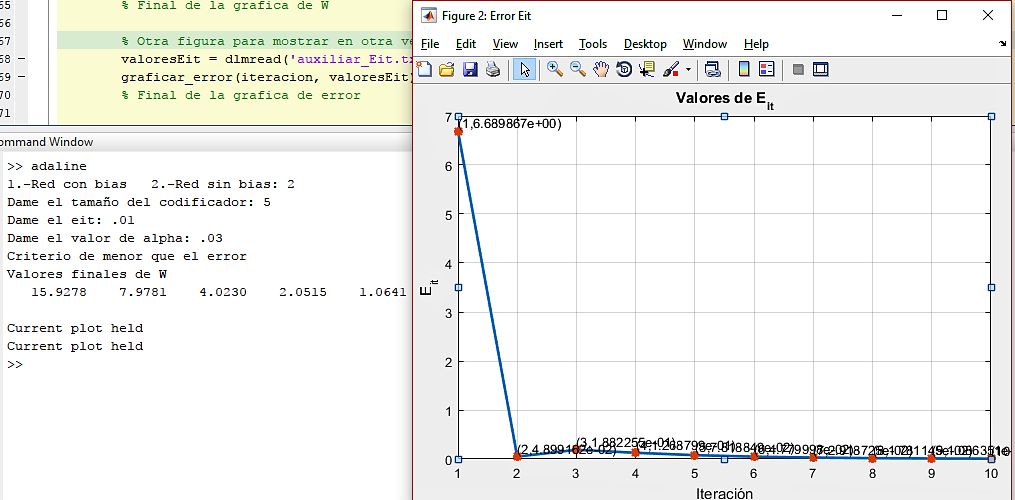
\includegraphics[width=16cm]{img/adaline4/error.png}
            \caption{Prueba 2 de ADALINE sin bias.}
            \label{fig:adaline4error}
        \end{center}
    \end{figure}
    La red convergió en la debido a que el error es menor al valor aceptable dando como resultado los siguientes valores de $\boldsymbol{W}$.
    \[ \boldsymbol{W} = \left[\begin{array}{ccccc}15.9278 & 7.9781 & 4.023 & 2.0515 & 1.0641\end{array}\right] \]
    \begin{figure}[H]
        \begin{center}
            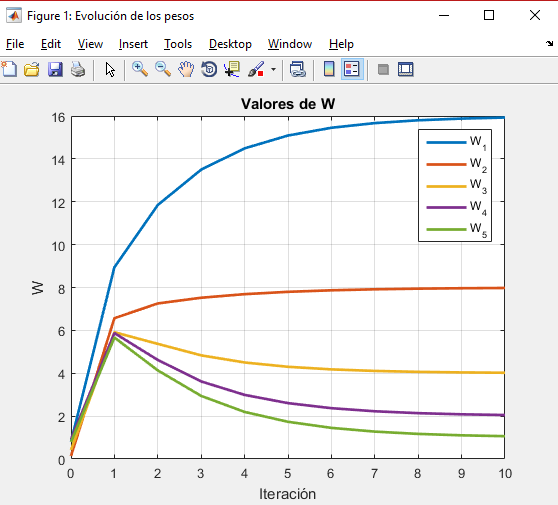
\includegraphics[width=10cm]{img/adaline4/pesosbias.png}
            \caption{Pesos de esta prueba.}
            \label{fig:adaline4pesos}
        \end{center}
    \end{figure}
\newpage
    \section{Discusión de resultados}
    Respecto a los experimentos realizados en ADALINE sin bias podemos observar que entre mayor sea el tamaño del codificador a trabajar a la red le toma más iteraciones converger a un resultado. Además por las gráficas \ref{fig:adaline3error} y \ref{fig:adaline4error} podemos observar que el error tiende a disminuir bastante rápido en las primeras iteraciones para después pasar a hacerlo de una forma más lenta hasta alcanzar un valor aceptable.
    
    De igual forma los pesos en estos dos experimentos crecen a un ritmo similar en las primeras iteraciones para después tender a estabilizarse en valores diferentes, para este punto no hay un comportamiento claro ya que algunos valores empiezan a crecer mientras otros decrecen pero algo que tienen en común es que en las ultimas iteraciones estos ya no sufren demasiados cambios lo cual es obvio por la gráfica de la evolución del error.
    
    En ADALINE con bias la historia se repite ya que los comportamientos de las gráficas son bastante similares a su contraparte sin bias, suceden cambios drásticos en las primeras iteraciones para después proceder a hacer pequeños ajustes en las ultimas iteraciones.
    \newpage
    \section{Conclusiones}
    % Ventajas, desventajas y discutir resultados
    Lo primero que podemos observar en en los resultados es la ventaja que tiene la red ADALINE con respecto al perceptron debido a su regla de aprendizaje (LMS) sin embargo esto solo se puede aprovechar debido a que los problemas que probamos fueron linealmente separables, en caso contrario al igual que con el perceptron no podríamos llevar a cabo esta distinción entre clases sin embargo ADALINE no tiene el problema que sufre el perceptron con el ruido.
    \\\\
    Es por esto que es importante mencionar su importancia en el procesamiento de señales donde nos permite predecir el valor de una señal en un tiempo $t+1$ con base a los $p$ instantes anteriores (filtros adaptativos) y en la eliminación de ruido en señales portadoras información.
    \\\\
    El hecho de que la salida de la red sea un valor real y no solo que nos diga si nos equivocamos o no como en el caso del perceptron es lo que nos permite saber cuanto se ha equivocado y poder hacer que nuestro aprendizaje sea mejor.
    
    Otra gran ventaja que nos brinda ADALINE es el hecho de que podemos indicar el factor de aprendizaje y con ello regular la modificación de los pesos y no tener cambios demasiados bruscos que pudieran causar que el error en lugar de disminuir, aumentara.
    \newpage
    \bibliographystyle{apalike}
    \bibliography{bibliografia}
    \newpage
    \section{Anexo}
\begin{lstlisting}
%% Funcion principal
function adaline()
    opcion = input('1.-Red con bias   2.-Red sin bias: ', 's');
    if str2double(opcion) == 1
        adaline_bias();
    else
        % Captura de los datos
        tam = input('Dame el tam del codificador: ', 's');
        tam = str2double(tam);
        tabla_verdad = zeros(2^tam, tam+1);
        eit = input('Dame el eit: ', 's');
        eit = str2double(eit);
        alpha = input('Dame el valor de alpha: ', 's'); % 0.3
        alpha = str2double(alpha);
        N = 2^tam-1;
        W = rand(1, tam);
        auxiliar_w = fopen('auxiliar_w.txt', 'w');
        auxiliar_Eit = fopen('auxiliar_Eit.txt', 'w');
        fprintf(auxiliar_w, '%.10f ', W);
        fprintf(auxiliar_w, '\n');
        % Llenamos nuestra tabla de verdad
        for i = 0:N
            a = dec2bin(i, tam) - '0';
            tabla_verdad(i+1, 1:tam) = a;
            tabla_verdad(i+1, tam+1) = i;
        end;
        continuar = true;
        iteracion = 1;
        while continuar
            Eit = 0;
            for n = 1:N
                p = tabla_verdad(n, 1:tam)';
                a = purelin(W*p);
                t = tabla_verdad(n, tam+1);
                ed = t-a;
                Eit = Eit + ed;
                W = W + (2 * alpha * ed*p');
            end
            Eit = 1/N * Eit;
            Eit = abs(Eit);
            fprintf(auxiliar_Eit, '%.10f ', Eit);
            fprintf(auxiliar_Eit, '\n');
            
            fprintf(auxiliar_w, '%.10f ', W);
            fprintf(auxiliar_w, '\n');
            if Eit == 0
                disp('Criterio de igualdad a cero');
                break;
            elseif Eit < eit
                disp('Criterio de menor que el error');
                break;
            end
            iteracion = iteracion + 1;
        end
        fclose(auxiliar_Eit);
        fclose(auxiliar_w);
        
        % Desplegar los valores finales
        disp('Valores finales de W');
        disp(W);
        
        % Figura de los valores de W
        valoresW = dlmread('auxiliar_w.txt');
        graficar_pesos(tam, valoresW, iteracion);
        % Final de la grafica de W
        
        % Otra figura para mostrar en otra ventana
        valoresEit = dlmread('auxiliar_Eit.txt');
        graficar_error(iteracion, valoresEit)
        % Final de la grafica de error
        
        % Guardamos en un archivo
        a_final = strcat('resultado_', datestr(now, 'HH-MM_dd-mm-yyyy'));
        a_final = strcat(a_final, '.txt');
        valores_finales = fopen(a_final, 'w');
        fprintf(valores_finales, 'Valores finales de W \n');
        fprintf(valores_finales, '%.10f ', W);
        fprintf(valores_finales, '\n');
        fclose(valores_finales);
    end
end % Final de la funcion principal
    
%% graficar_pesos: function description
function graficar_pesos(tam, valoresW, iteracion)
    figure('Name', 'Evolucion de los pesos');
    % Grafica un vector en x y otro vector en y
    plot(0:iteracion, valoresW, 'LineWidth', 2); 
    hold;
    grid;
    % Etiquetas de los ejes
    xlabel('Iteracion');
    ylabel('W');
    
    % Titulo de nuestra grafica
    etiquetas = cell(1, tam);
    for i = 1:tam
        etiquetas{i} = ['W_' num2str(i)];
    end;
    legend(etiquetas);
    title('Valores de W');
end

%% graficar_error: function description
function graficar_error(iteracion, valoresEit)
    figure('Name', 'Error Eit');
    x = 1:iteracion;
    % Grafica un vector en x y otro vector en y
    plot(x, valoresEit, 'LineWidth', 2);
    hold;
    plot(x, valoresEit, '*', 'LineWidth', 2);
    grid;
    % Imprime las coordenadas de Eit
    strValues = strtrim(cellstr(num2str([x(:) valoresEit(:)], '(%d,%d)')));
    text(x, valoresEit, strValues, 'VerticalAlignment', 'bottom');
    % Etiquetas de los ejes
    xlabel('Iteracion');
    ylabel('E_{it}');
    % Titulo de nuestra grafica
    title('Valores de E_{it}');
end

%Con bias
function adaline_bias()
    archivo = input('Dame el nombre del archivo: ', 's');
    prueba = fopen(archivo, 'r');
    S = 0;
    targets = [];
    prototipos = [];
    R = 0;
    dimen = [];
    tipo_lectura = 0;
    while feof(prueba) == 0
        linea = fgetl(prueba);
        if linea ~= '{'
            fclose(prueba);
            datos = dlmread(archivo);
            tam = size(datos);
            S = 1;
            prototipos = datos(:, 1:tam(2)-1)';
            dimen = size(prototipos);
            targets = datos(:, tam(2))';
            R = dimen(1);
            tipo_lectura = 1;
            break;
        else
            linea = linea(2:length(linea)-1);
            proto = linea(2:find(linea==',')-2);
            tar = linea(find(linea==',')+2:length(linea)-1);
            proto = str2num(proto);
            tar = str2num(tar);
            prototipos = [prototipos proto'];
            targets = [targets tar'];
        end
    end
    if tipo_lectura == 0
        S = 2;
        dimen = size(prototipos);
        R = dimen(1);
    end   
    itmax = input('Ingrese valor de itmax: ', 's'); %5
    itmax = str2double(itmax);
    alpha = input('Dame el valor de alpha: ', 's'); % 0.3
    alpha = str2double(alpha);
    eit = input('Dame el eit: ', 's');
    eit = str2double(eit);
    W = ones(S, R);
    b = ones(S, 1);
    
    auxiliar_w = fopen('auxiliar_w.txt', 'w');
    auxiliar_bias = fopen('auxiliar_bias.txt', 'w');
    auxiliar_error = fopen('auxiliar_Eit.txt', 'w');
    fprintf(auxiliar_w, '%.10f ', W);
    fprintf(auxiliar_w, '\n');
    
    fprintf(auxiliar_bias, '%.10f ', b);
    fprintf(auxiliar_bias, '\n');
    criterio = 0;
    for iteracion = 1:itmax
        Eit = 0;
        for n = 1:dimen(2)
            p = prototipos(:, n);
            a = purelin(W*p + b);
            t = targets(:, n);
            ed = t-a;
            Eit = Eit + ed;
            W = W + (2 * alpha * ed * p');
            b = b + (2 * alpha * ed);
        end
        Eit = 1/dimen(2) * Eit;
        Eit = abs(Eit);
        fprintf(auxiliar_error, '%.10f ', Eit);
        fprintf(auxiliar_error, '\n');
        
        fprintf(auxiliar_w, '%.10f ', W);
        fprintf(auxiliar_w, '\n');
        
        fprintf(auxiliar_bias, '%.10f ', b);
        fprintf(auxiliar_bias, '\n');
        if Eit == 0
            criterio = 1;
            break;
        elseif Eit < eit
            criterio = 2;
            break;
        end
    end
    fclose(auxiliar_error);
    fclose(auxiliar_w);
    fclose(auxiliar_bias);
    
    % Figura de los valores de W
    valoresW = dlmread('auxiliar_w.txt');
    valores_bias = dlmread('auxiliar_bias.txt');
    graficar_pesos_bias(valoresW, iteracion, S, R);
    graficar_bias(valores_bias, iteracion, S);
    % Final de la grafica de W
    
    % Otra figura para mostrar en otra ventana
    valoresEit = dlmread('auxiliar_Eit.txt');
    graficar_error_bias(iteracion, valoresEit, S);
    % Final de la grafica de error
    
    if criterio == 0
        disp('Termino alcanzando el maximo de iteraciones')
    elseif criterio == 1
        disp('Termino por criterio de error igual a 0');
        fprintf('Termino en la iteracion %d\n', iteracion);
        disp('Valores finales de W:');
        disp(W);
        disp('Valores finales del bias:');
        disp(b);
    else
        disp('Termino por criterio de menor al error permitido');
        fprintf('Termino en la iteracion %d\n', iteracion);
        disp('Valores finales de W:');
        disp(W);
        disp('Valores finales del bias:');
        disp(b);
    end
    
    archivo_final = strcat('resultado_', datestr(now, 'HH-MM_dd-mm-yyyy'));
    archivo_final = strcat(archivo_final, '.txt');
    finales = fopen(archivo_final, 'w');
    fprintf(finales, 'Valores finales de W: \n');
    fprintf(finales, '%.10f ', W);
    fprintf(finales, '\n');
    
    fprintf(finales, 'Valores finales del bias: \n');
    fprintf(finales, '%.10f ', b);
    fprintf(finales, '\n');
    fclose(finales);
end


%% graficar_pesos: function description
function graficar_pesos_bias(valoresW, iteracion, S, R)
    figure('Name', 'Evolucion de los pesos');
    % Grafica un vector en x y otro vector en y
    plot(0:iteracion, valoresW, 'LineWidth', 2); 
    hold;
    grid;
    % Etiquetas de los ejes
    xlabel('Iteracion');
    ylabel('W');
    
    etiquetas = cell(1, S*R);
    k = 1;
    for i = 1:S
        for j = 1:R
        etiquetas{k} = ['W_{' num2str(i) ',' num2str(j) '}'];
        k = k+1;
        end;
    end;
    legend(etiquetas);
    title('Valores de W');
end

%% graficar_error: function description
function graficar_error_bias(iteracion, valoresEit, S)
    figure('Name', 'Error Eit');
    x = 1:iteracion;
    % Grafica un vector en x y otro vector en y
    plot(x, valoresEit, 'LineWidth', 2);
    hold;
    grid;
    % Etiquetas de los ejes
    xlabel('Iteracion');
    ylabel('E_{it}');
    % Titulo de nuestra grafica
    etiquetas = cell(1, S);
    for i = 1:S
        etiquetas{i} = ['Neurona ' num2str(i)];
    end;
    legend(etiquetas);
    % Titulo de nuestra grafica
    title('Valores de E_{it}');
end

%% graficar_bias
function graficar_bias(valores_bias, iteracion, S)
    figure('Name', 'Evolucion del bias');
    % Grafica un vector en x y otro vector en y
    plot(0:iteracion, valores_bias, 'LineWidth', 2); 
    hold;
    grid;
    % Etiquetas de los ejes
    xlabel('Iteracion');
    ylabel('Bias');
    % Titulo de nuestra grafica
    etiquetas = cell(1, S);
    for i = 1:S
        etiquetas{i} = ['b_' num2str(i)];
    end;
    legend(etiquetas);
    title('Valores del bias');
end
\end{lstlisting}
\end{document}